\mychapter{1}{Lesson 1} %180926

Talking cryptography is usually done in the ``confidentiality'' realm, where two characteristics in a communication channel are desirable: it must be \emph{secret}, and \emph{authentic}.

Modern confidentiality/authentication systems are forged under \emph{Kerckhoffs's principle}, which states that a secure system shall only rely on the encryption keys, and not on the underlying algorithm's secrecy; in short, \emph{``No security by obscurity''}. However sharing the key between two parties without the risk of eavesdropping is a costly operation.

\section{Secret communication}

\todo{Image of Alice, Bob, Eve in ske}

The typical objects defined and used in secret communication topics are:
\begin{itemize}
    \item $\K$: Key space
    \item $\M$: Message space
    \item $\C$: Ciphertext space
    \item $\Enc \in \K \times \M \to \C$: Encryption routine
    \item $\Dec \in \K \times \C \to \M$: Decryption routine
\end{itemize}

\Enc{} and \Dec{} form a \emph{cryptographic secrecy scheme}, or just \emph{secrecy scheme} for brevity, and as such, it must abide by the rule:
\[
    \forall m \in \M, \forall k \in \K \implies \Dec(k, \Enc(k, m)) = m
\]

\begin{definition}
    (\textit{Shannon's ``Perfect secrecy''}): Let $M$ be any distribution over the message space $\M$, and $K$ a uniform distribution over $\K$. Then, the cryptosystem $\Xi: (\Enc, \Dec)$ is deemed \emph{perfectly secret} iff the ciphertext obtained by applying the encryption routine to a message sampled by $M$ using tke key in $K$ is effectively useless in retrieving any info about the message itself, apart from the key-supplied decryption routine. Formally:
    \[
        \forall M \sim \mathcal{R}and(\M),\, \forall C \sim \mathcal{R}and(\C) \implies \Pr[M = m] = \Pr[M = m \knowing C \evaluatesto c]
    \]
\end{definition}
Note how this definition doesn't involve the encryption key. % Is it important? Why?

The perfect secrecy definition can be rephrased in different ways, bringing more details to light:
\begin{enumerate}
    \item \label{def:ps1} $\Pr[M = m] = \Pr[M = m \knowing C \evaluatesto c]$
    \item \label{def:ps2}$M \indep C$
    %TODO - Better formalize: the variables m, m' and k are 'chosen' by their own distibutions, c is just a result instead
    % Maybe decompose it into smaller bits: use event sets instead
    \item \label{def:ps3}$\forall m_1, m_2 \in \M, c \in \C \implies \Pr[\Enc(K, m_1) = c] = \Pr[\Enc(K, m_2) = c]$
\end{enumerate}
    
\begin{proposition}
    All the previous statements are equivalent.
\end{proposition}

\begin{proof}
    The proof is structured as a cyclic implication between the three definitions:
    
    \begin{itemize}
        \item $(\ref{def:ps1}) \implies (\ref{def:ps2})$: Start from one side of the independency ddefinition, and work through the other:
        \begin{align*}
            & \Pr[C = c \wedge M = m]                           & \\
            =& \Pr[C = c] \Pr[M = m \knowing C \evaluatesto c]  & \text{(Conditioned prob.)} \\
            =& \Pr[C = c] \Pr[M = m]                            & \text{(Using 1.)} \\
        \end{align*}
        This proves that $M$ and $C$ are independent distributions.
        
        \item $(\ref{def:ps2}) \implies (\ref{def:ps3})$: For the proof's purposes, let $M$ be an arbitrary distribution over $\M$; recall that, by definition: $C := \Enc(K, M)$:
        \begin{align*}
            & \Pr[\Enc(K, m_1) = c]                             & \\
            =& \Pr[\Enc(K, M) = c \knowing M \evaluatesto m_1]  & \text{(Introducing $M$)} \\
            =& \Pr[C = c \knowing M \evaluatesto m_1]           & \text{($C$ defintion)} \\
            =& \Pr[C = c]                                       & \text{(Using 2.)} \\
            =& \dots                                            & \mathllap{\text{(Same steps reversed, where $m_1 \mapsto m_2$)}} \\
            =& \Pr[\Enc(K, m_2) = c]                            & \\
        \end{align*}


        \item $(\ref{def:ps3}) \implies (\ref{def:ps1})$:
        \begin{align*}
            & \Pr[C = c] & \\
            =& \sum_{m}\Pr[C = c \wedge M = m]                                  & \text{(Total prob.)} \\
            =& \sum_{m}\Pr[\Enc(K, M) = c \wedge M = m]                         & \text{($C$ definition)} \\
            =& \sum_{m}\Pr[\Enc(K, M) = c \knowing M \evaluatesto m] \Pr[M = m] & \text{(Cond. prob. def.)} \\
            =& \sum_{m}\Pr[\Enc(K, m) = c] \Pr[M = m]                           & \text{(Cond. collapse)} \\
            =& \Pr[\Enc(K, \overline{m}) = c] \sum_{m} \Pr[M = m]               & \text{(Using 3.)} \\ %TODO Not convinced thoroughly
            =& \Pr[\Enc(K, \overline{m}) = c]                                   & \text{(Total prob.)} \\
            =& \Pr[\Enc(K, M) = c \knowing M \evaluatesto \overline{m}]         & \text{(Introducing $M$)} \\
            =& \Pr[C = c \knowing M \evaluatesto \overline{m}]                  & \text{($C$ definition)} \\
        \end{align*}

        Knowing this, and applying Bayes' theorem, we get back to the first definition:
        \begin{align*}
            & \Pr[C = c] = \Pr[C = c \knowing M \evaluatesto m]                                         & \\
            \implies& \Pr[C = c] = \Pr[M = m \knowing C \evaluatesto c] \frac{\Pr[C = c]}{\Pr[M = m]}   & \text{(Bayes' theorem)} \\
            \implies& \Pr[M = m] = \Pr[M = m \knowing C \evaluatesto c]                                 & \\
        \end{align*}

    \end{itemize}

    Thus, we conclude that all three definitions for perfect secrecy are equivalent.

\end{proof}

A remark on definition \ref{def:ps3} has to be done here:

\begin{align*}
    & \Pr[\Enc(K, m) = c] \\
    =& \Pr[\Enc(K, M) = c \knowing M \evaluatesto m] \\
    \neq& \Pr[\Enc(K, M) = c]
\end{align*}

which is exactly the difference between picking a specific message $m$ (as in: \emph{choosing} $m$), and picking it at random, just as $M$ denotes implicitly.

\subsection{One Time Pad (OTP)}

Let $\K = \M = \C = \binary^l$, and define the following cryptographic scheme:
\begin{itemize}
    \item $\Enc(k, m) = k \xor m = c$
    \item $\Dec(k, c) = k \xor c = m$
\end{itemize}

Proof of correctness goes like: $\Dec(k, \Enc(k, m)) = \Dec(k, k \xor m) = k \xor k \xor m = m$.

\begin{theorem}
    The \emph{One-time pad} scheme is perfectly secret.
\end{theorem}
\begin{proof}
    Let $K \sim \unifdist(\K)$. Then, $\forall m_1, m_2, c \in \binary^l$:
    \begin{align*}
        & \Pr[\Enc(K, m_1) = c]     & \\
        =& \Pr[K \xor m_1 = c]      & \\
        =& \Pr[K = c \xor m_1]      & \\
        =& |\K|^{-1}                & \text{(K is uniform)} \\
        =& \dots                    & \text{(Same steps reversed, where $m_1 \mapsto m_2$)} \\
        =& \Pr[\Enc(K, m_2) = c]    & \\  
    \end{align*}
    This satisfies the third definition of perfect secrecy.
\end{proof}

%TODO OLD NOTE: Observation: k is truly random, but fixed, compare with Pi_\xor's encryption routine: from a security standpoint, nothing changes! actualy, \Pi_\xor may be weaker bruteforce wise than OTP!

By observing our recent proof, some insights (and problems) arise:
\begin{enumerate}
    \item The key and the message's lengths must always match ($|k| = |m|$);
    \item As the name suggests, keys are useful just for one encryption. Otherwise, given two encryptions witht he same key, an attacker may exploit the \textsc{xor}'s idempotency to extract valuable information from both ciphertexts\footnote{This vulnerability of applying a function on a ciphertext, and expecting as a result the image of the original message by the same function, is called \emph{malleability}, and is explored further in the notes.}:
    \[
        c_1 = k \xor m_1 \wedge c_2 = k \xor m_2 \implies c_1 \xor c_2 = m_1 \xor m_2
    \]
    
\end{enumerate}

%\footnote{An encryption algorithm is "malleable" if it is possible to transform a ciphertext into another ciphertext which decrypts to a related plaintext. That is, given an encryption $c$ of a plaintext $m$, it is possible to generate another valid ciphertext $c'$, for a known $Enc$, $Dec$, without necessarily knowing or learning $m$.}

Combined with the fact that keys must be preemptively shared in a secure fashion, these problems make for a quite impractical cryptographic scheme. One can further this analysis and generalize it to all ``perfect'' schemes, giving a rather delusive conclusion:

\begin{figure}[h]
    \centering
    \def\firstcircle{(0,0) circle (1.5cm)}
    \def\secondcircle{(60:0) circle (0.9cm)}
    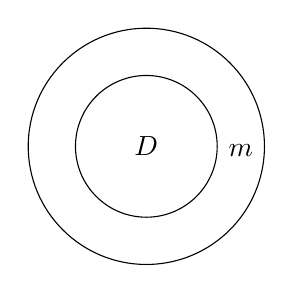
\begin{tikzpicture}
        \begin{scope}[shift={(3cm,-5cm)}]
            \draw \firstcircle node[label={[xshift=1.0cm, yshift=0.3cm]$\M$}] { };
            \draw \secondcircle node[label={[xshift=1.2cm, yshift=-0.5cm]$m$}] {$D$};
        \end{scope}
    \end{tikzpicture}
    \caption{Where the messages stand}
\end{figure}

\begin{theorem}
    For a secrecy scheme to be perfectly secret: $|\K| \geq |\M|$
\end{theorem}
\begin{proof}
    Perfection will be disproved by breaking definition \ref{def:ps1}. Let $M \sim \unifdist(\M)$, and take $c \in \C : \Pr[C = c] > 0$. Consider $D = \{\Dec(k, c) : k \in \K\}$ as the set of all images of the decryption routine with all keys in $\K$. The offending assumption is that $|\K| < |\M|$. Then, by how $D$ is defined:

    \[
        |D| \leq |\K| < |\M| \implies \exists m \in \M \setminus D
    \]

    Fix this message $m$, and remember that by $M$'s definition, $\Pr[M = m] = |\M|^{-1}$. Since $m \notin D$, there can be no key in $\K$ such that $\Dec(k, c) = m$. By observing that $C$ strictly distributes over $D$, where $m$ is not present, $\Pr[M = m \knowing C \evaluatesto c] = 0$. Putting everything together:
    \[
        0 = \Pr[M = m \knowing C \evaluatesto c] \neq \Pr[M = m] = |\M|^{-1}
    \]
    This clearly violates the first definition of perfect secrecy.
\end{proof}
